\documentclass[letter]{revtex4}
\usepackage[utf8]{inputenc}

\usepackage{epsfig}
\usepackage{graphicx}
\usepackage{tikz}
\usetikzlibrary{shapes.geometric, arrows}
\graphicspath{ {images/} }
\usepackage{listings}
\usepackage{color}
\usepackage{amsmath}


\usepackage{xcolor}

\definecolor{codegreen}{rgb}{0,0.6,0}
\definecolor{codegray}{rgb}{0.5,0.5,0.5}
\definecolor{codepurple}{rgb}{0.58,0,0.82}
\definecolor{backcolour}{rgb}{0.95,0.95,0.92}

\lstdefinestyle{mystyle}{
    backgroundcolor=\color{backcolour},   
    commentstyle=\color{codegreen},
    keywordstyle=\color{magenta},
    numberstyle=\tiny\color{codegray},
    stringstyle=\color{codepurple},
    basicstyle=\ttfamily\footnotesize,
    breakatwhitespace=false,         
    breaklines=true,                 
    captionpos=b,                    
    keepspaces=true,                 
    numbers=left,                    
    numbersep=5pt,                  
    showspaces=false,                
    showstringspaces=false,
    showtabs=false,                  
    tabsize=2
}

\lstset{style=mystyle}


\begin{document}

\title{Práctica 2: Calculadora de Matrices}
\author{Archundia Bazán Aarón Antonio, Guerrero Velez Eliseo Milton, Hernández Vázquez Cesar Arturo}
\affiliation{Unidad Profesional Interdisciplinaria en Ingenier\'{\i}a y Tecnolog\'{\i}as Avanzadas del I.P.N.\\ Ingeniería Biónica,Programación Orientada a Objetos}

\date{23 de octubre de 2020}
\maketitle


\section{Planteamiento del problema}

El problema consiste en desarrollar una calculadora de matrices que trabaje con las siguientes operaciones para matrices bidimensionales de cualquier tamaño: 
\begin{itemize}
    \item Suma
    \item Resta
    \item Multiplicación
    \item Transpuesta
\end{itemize}
Donde el tamaño de la matriz sea dado por el usuario y respete las propiedades matrices así como las reglas para cada uno de los métodos antes propuestos.

\section{Propuesta de Solución}
Para dar una solución a este problema hay que revisar cuales con las que se tiene que trabajar este sistema. En este caso las propiedades para las operaciones con  matrices.  \\ 
  \textbf{Matriz:} \\
  Una matriz A de \emph{m} $\times$ \emph{n}  un arreglo rectangular \emph{mn} números dispuestos en \emph{m} renglones y \emph{n} columnas.
  
  
   $$ A=
       \begin{pmatrix}
        a_{11} & a_{12} & \cdots & a_{1n}\\
        a_{21} & a_{22} & \cdots & a_{2n}\\
        \vdots & \vdots & \ddots & \vdots\\
        a_{m1} & a_{m2} & \cdots & a_{mn}
    \end{pmatrix}
    $$
\textbf{Suma de matrices: }\\
La suma de dos matrices se define únicamente cuando son del mismo tamaño. La suma de A y B está dada por A+B: 
   $$ A+B=
       \begin{pmatrix}
        a_{11}+b_{11} & a_{12}+b_{12} & \cdots & a_{1n}+b_{1n}\\
        a_{21}+b_{21} & a_{22}+b_{22} & \cdots & a_{2n}+b_{2n}\\
        \vdots & \vdots & \ddots & \vdots\\
        a_{m1}+b_{m1} & a_{m2}+b_{m2} & \cdots & a_{mn}+b_{mn}
    \end{pmatrix}
    $$
\textbf{Resta de matrices: }\\
La resta de dos matrices se define únicamente cuando son del mismo tamaño. La resta de A y B está dada por A-B: 
   $$ A-B=
       \begin{pmatrix}
        a_{11}-b_{11} & a_{12}-b_{12} & \cdots & a_{1n}-b_{1n}\\
        a_{21}-b_{21} & a_{22}-b_{22} & \cdots & a_{2n}-b_{2n}\\
        \vdots & \vdots & \ddots & \vdots\\
        a_{m1}-b_{m1} & a_{m2}-b_{m2} & \cdots & a_{mn}-b_{mn}
    \end{pmatrix}
    $$
\textbf{Multiplcación de Matrices: }
Sean dos matrices AB las propiedades que deben cumplir son las siguientes: 

    $ 
        C=AB=(c_{ij})m \times n
    $
    
    Donde cada elemento $c_{ij}$ está definido por: 
   $$c_{ij}=\sum_{r=1}^{n} a_{ir}b_{rj}$$
    
    
   $$ C=A*B=
       \begin{pmatrix}
        a_{11}+b_{11} & a_{12}+b_{12} & \cdots & a_{1n}+b_{1n}\\
        \vdots & \vdots & \ddots & \vdots\\
        a_{m1}+b_{m1} & a_{m2}+b_{m2} & \cdots & a_{mn}+b_{mn}
       \end{pmatrix}
       *
       \begin{pmatrix}
        a_{11}+b_{11} & a_{12}+b_{12} & \cdots & a_{1p}+b_{1p}\\
        \vdots & \vdots & \ddots & \vdots\\
        a_{n1}+b_{n1} & a_{n2}+b_{n2} & \cdots & a_{np}+b_{np}
       \end{pmatrix}
       
    $$
    
    $$
    C= \begin{pmatrix}
        a_{11}b_{11} +\cdots+ a_{1n}b_{n1} & \cdots & a_{11}b_{np}+\cdots+a_{1n}b_{np}\\
        \vdots & \vdots & \ddots \\
        a_{m1}b_{11} +\cdots+ a_{mn}b_{n1} & \cdots & a_{m1}b_{1p}+\cdots+a_{mn}b_{np}\\
       \end{pmatrix}
    $$
Dos matrices  se pueden multiplicar únicamete si el numero de columnas de la primera matriz es igual a la segunda  De otro modo, los vectores que forman el renglón i en A y la columna j de B no tendrán el
mismo número de componentes y el producto punto en la ecuación Dicho de otro modo,
las matrices A y B serán incompatibles bajo la multiplicación.\\

\textbf{Transpuesta de una matríz:  }
Sea A = ($a_{ij}$ ) una matriz de$ m \times n$. Entonces la transpuesta de A, que se escribe $A^T$, es
la matriz de $n \times m$ que se obtiene al intercambiar los renglones por las columnas de A.
De manera breve, se puede escribir $A^T$ ($a_{ij}$ ). En otras palabras

  \begin{center}
    
 Si $ A=
       \begin{pmatrix}
        a_{11} & a_{12} & \cdots & a_{1n}\\
        a_{21} & a_{22} & \cdots & a_{2n}\\
        \vdots & \vdots & \ddots & \vdots\\
        a_{m1} & a_{m2} & \cdots & a_{mn}
    \end{pmatrix}
    $, entonces  $ A^T=
       \begin{pmatrix}
        a_{11} & a_{21} & \cdots & a_{m1}\\
        a_{21} & a_{22} & \cdots & a_{m2}\\
        \vdots & \vdots & \ddots & \vdots\\
        a_{1n} & a_{2n} & \cdots & a_{mn}
    \end{pmatrix}
    $
    
    Simplemente se coloca el renglón i de A como la columna i de $A^T$ y la columna j de A
como el renglón j de $A^T$.
\end{center}

Por lo tanto con los datos anteriores la propuesta de  solución fue hacer una  función main con pocas lineas de código que contenga un switch que pregunte la operación a realizar, una vez seleccionada ejecutará la operación llamando a la función creada para cada caso de calculo de matrices, al finalizar un do-while determinará por medio de una entrada si el programa continua corriendo o si se quiere salir.  

\clearpage
\section{Análisis y diseño}

\subsection{Diagrama de flujo función main()}
\begin{center}
 	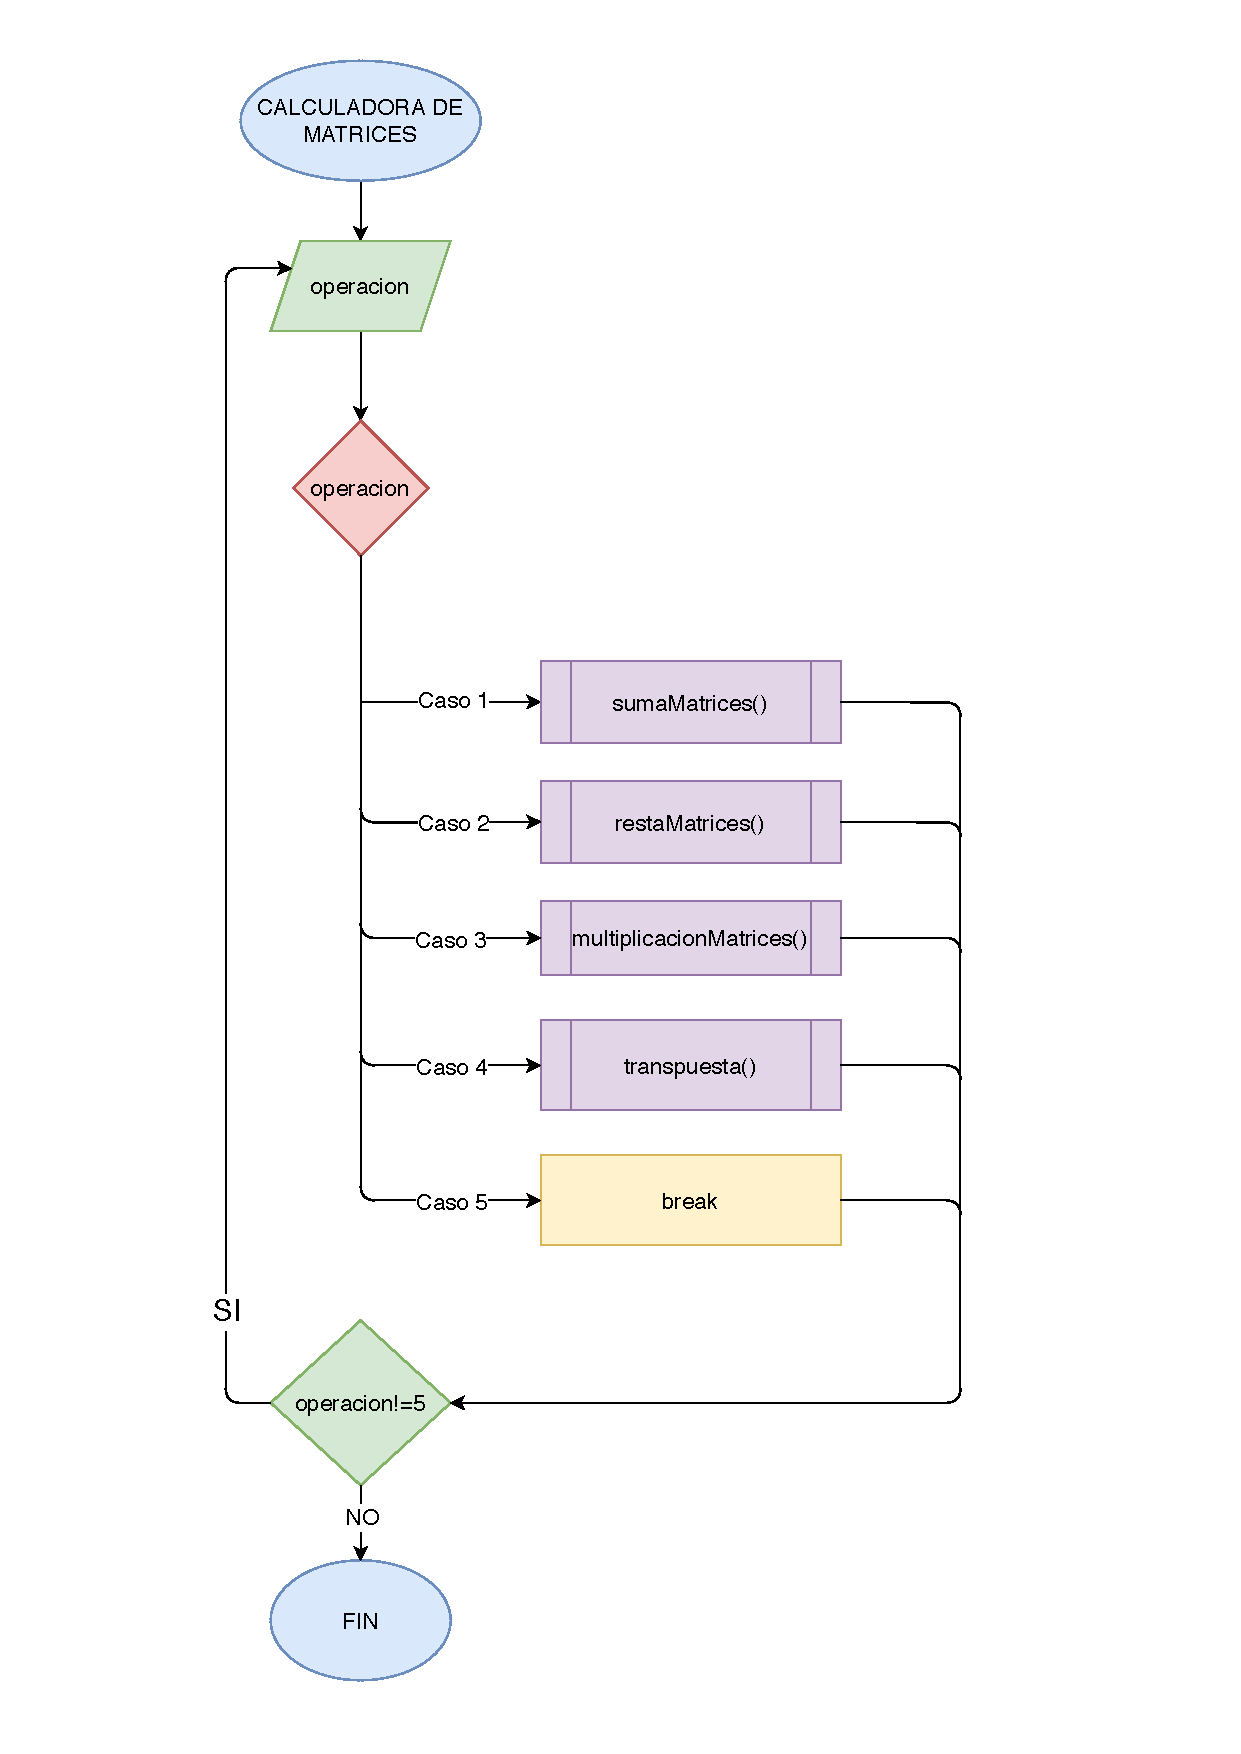
\includegraphics[scale=0.8]{Images/Practica2POO.pdf}
 	\captionof{Diagrama 1: }{Función Main()}
 	\label{figura4}
 \end{center}

\clearpage

\subsection{Diagrama función sumaMatrices ()}
\begin{center}
 	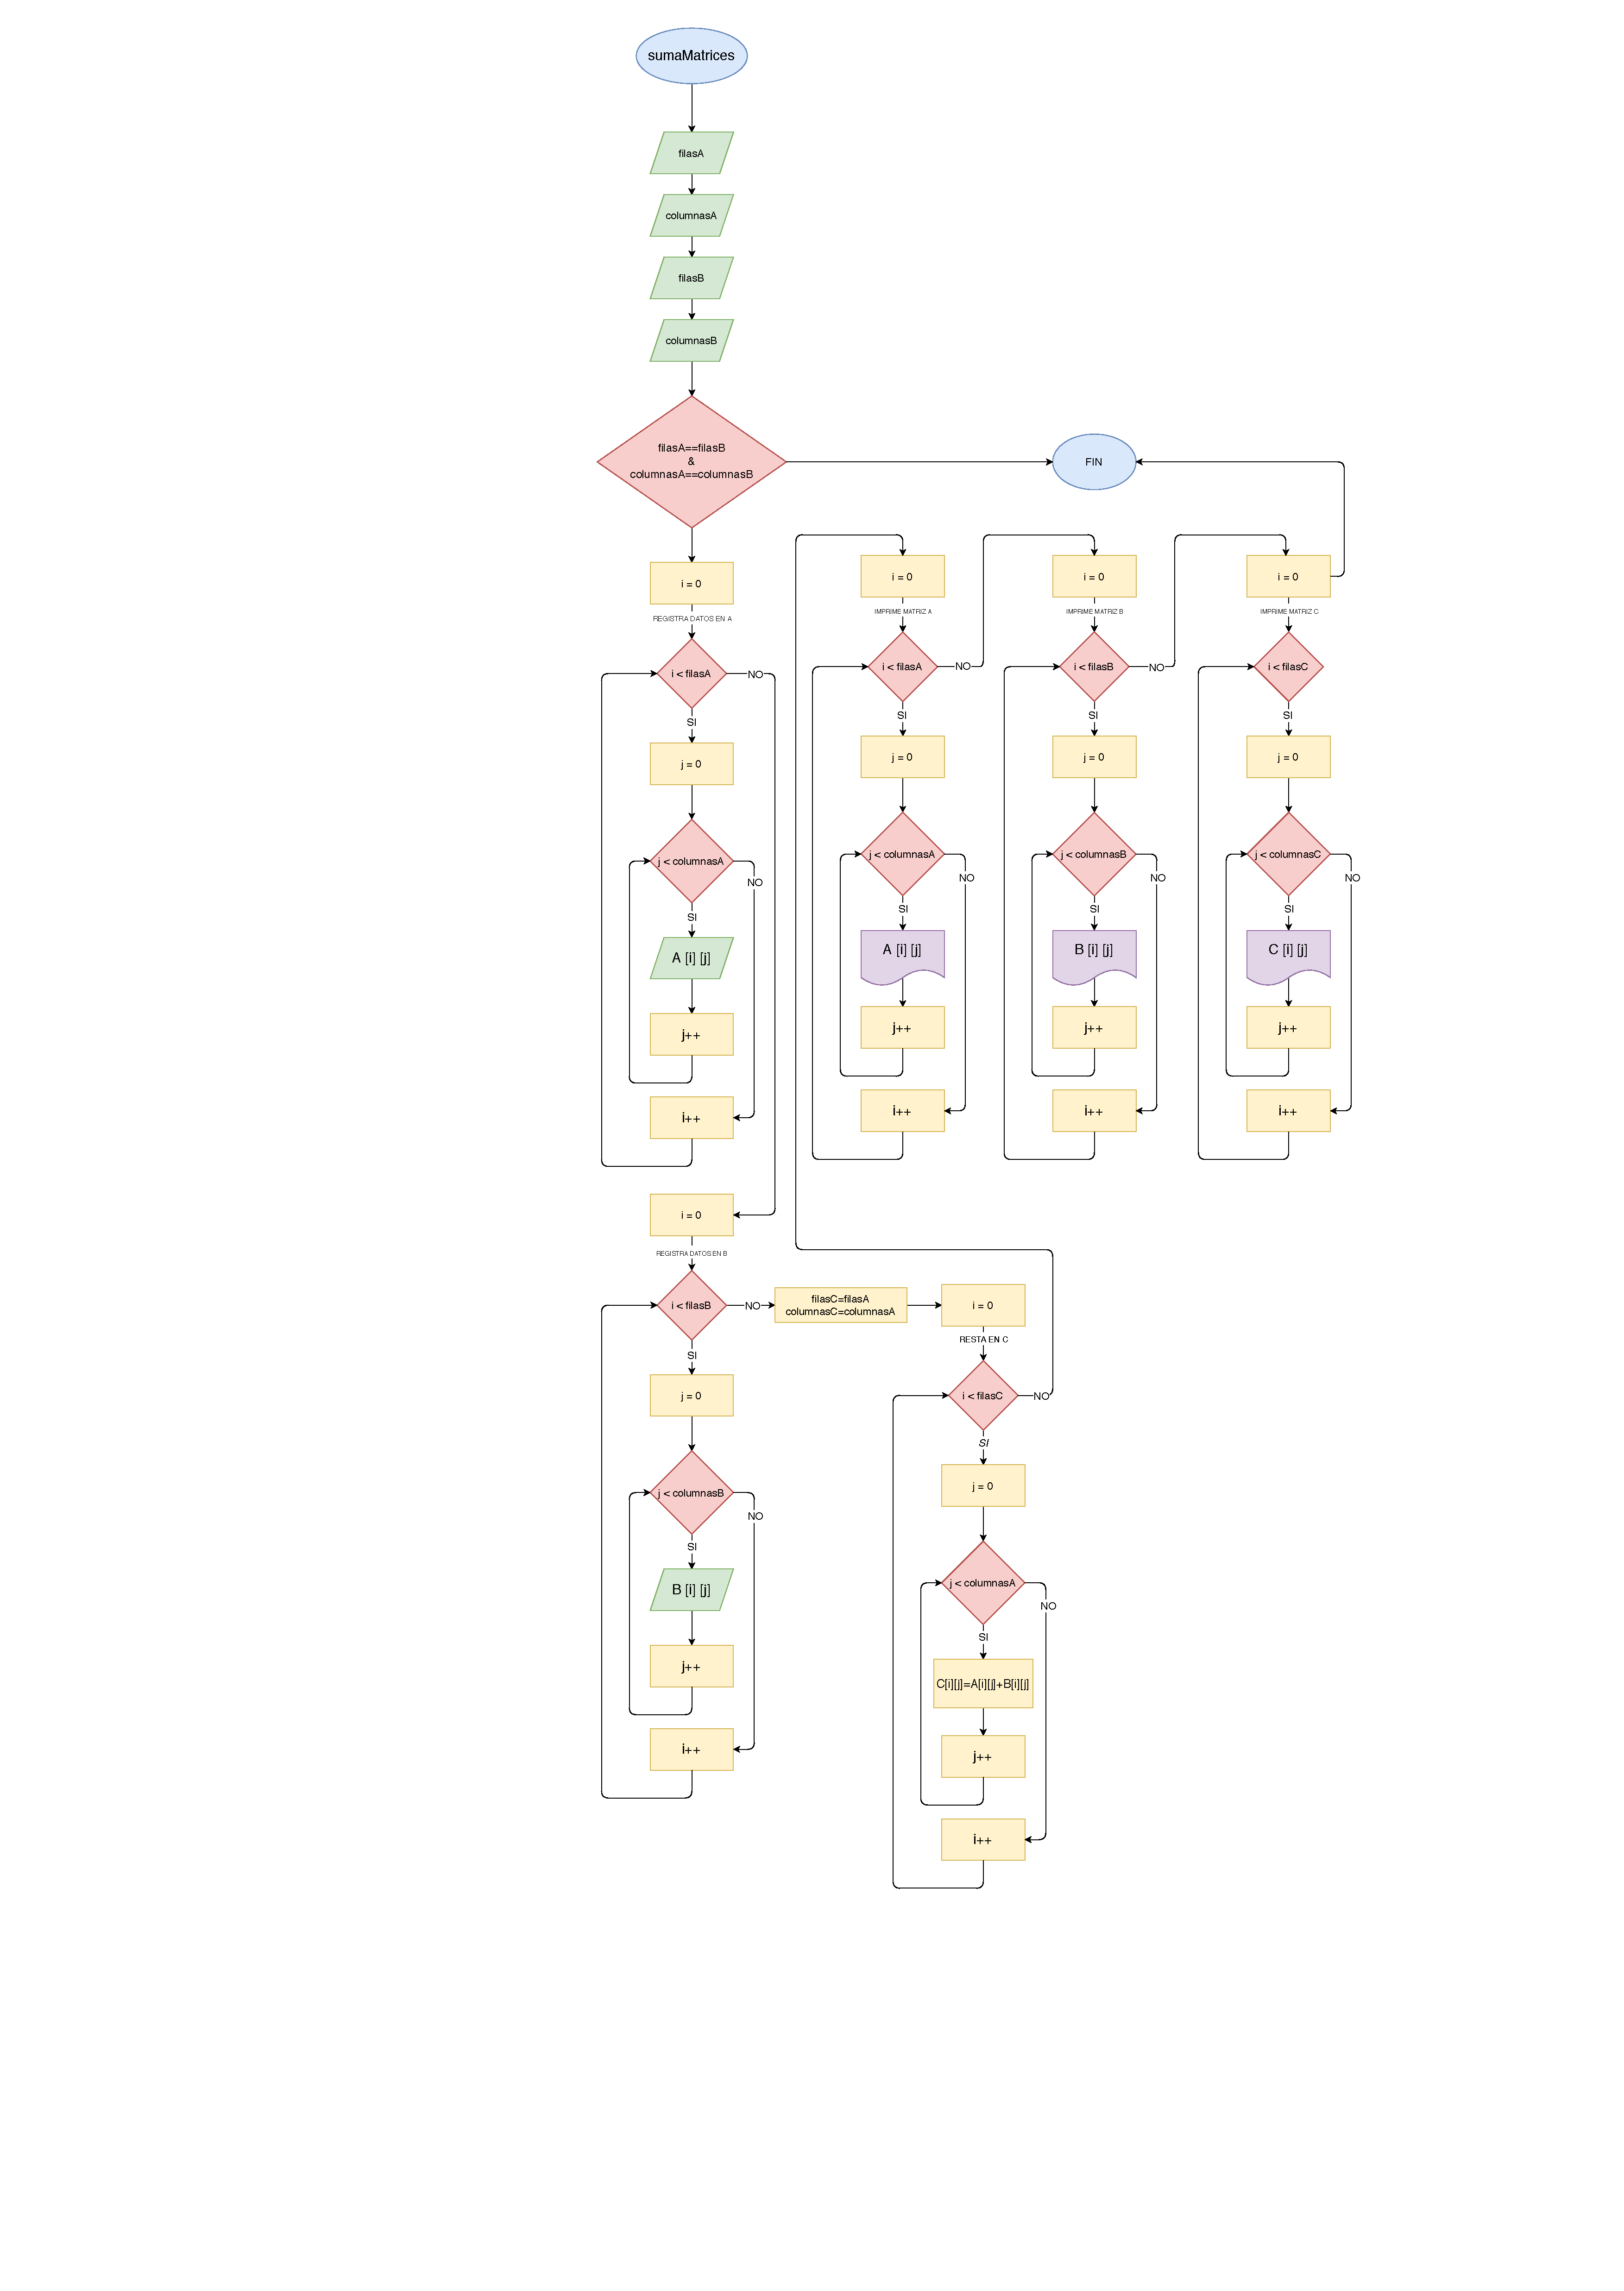
\includegraphics[scale=0.3]{Images/Suma.pdf}
 	\captionof{Diagrama 2: }{Función sumaMatrices()}
 	\label{figura4}
 \end{center}
\clearpage


\subsection{Diagrama función restaMatrices ()}

\begin{center}
 	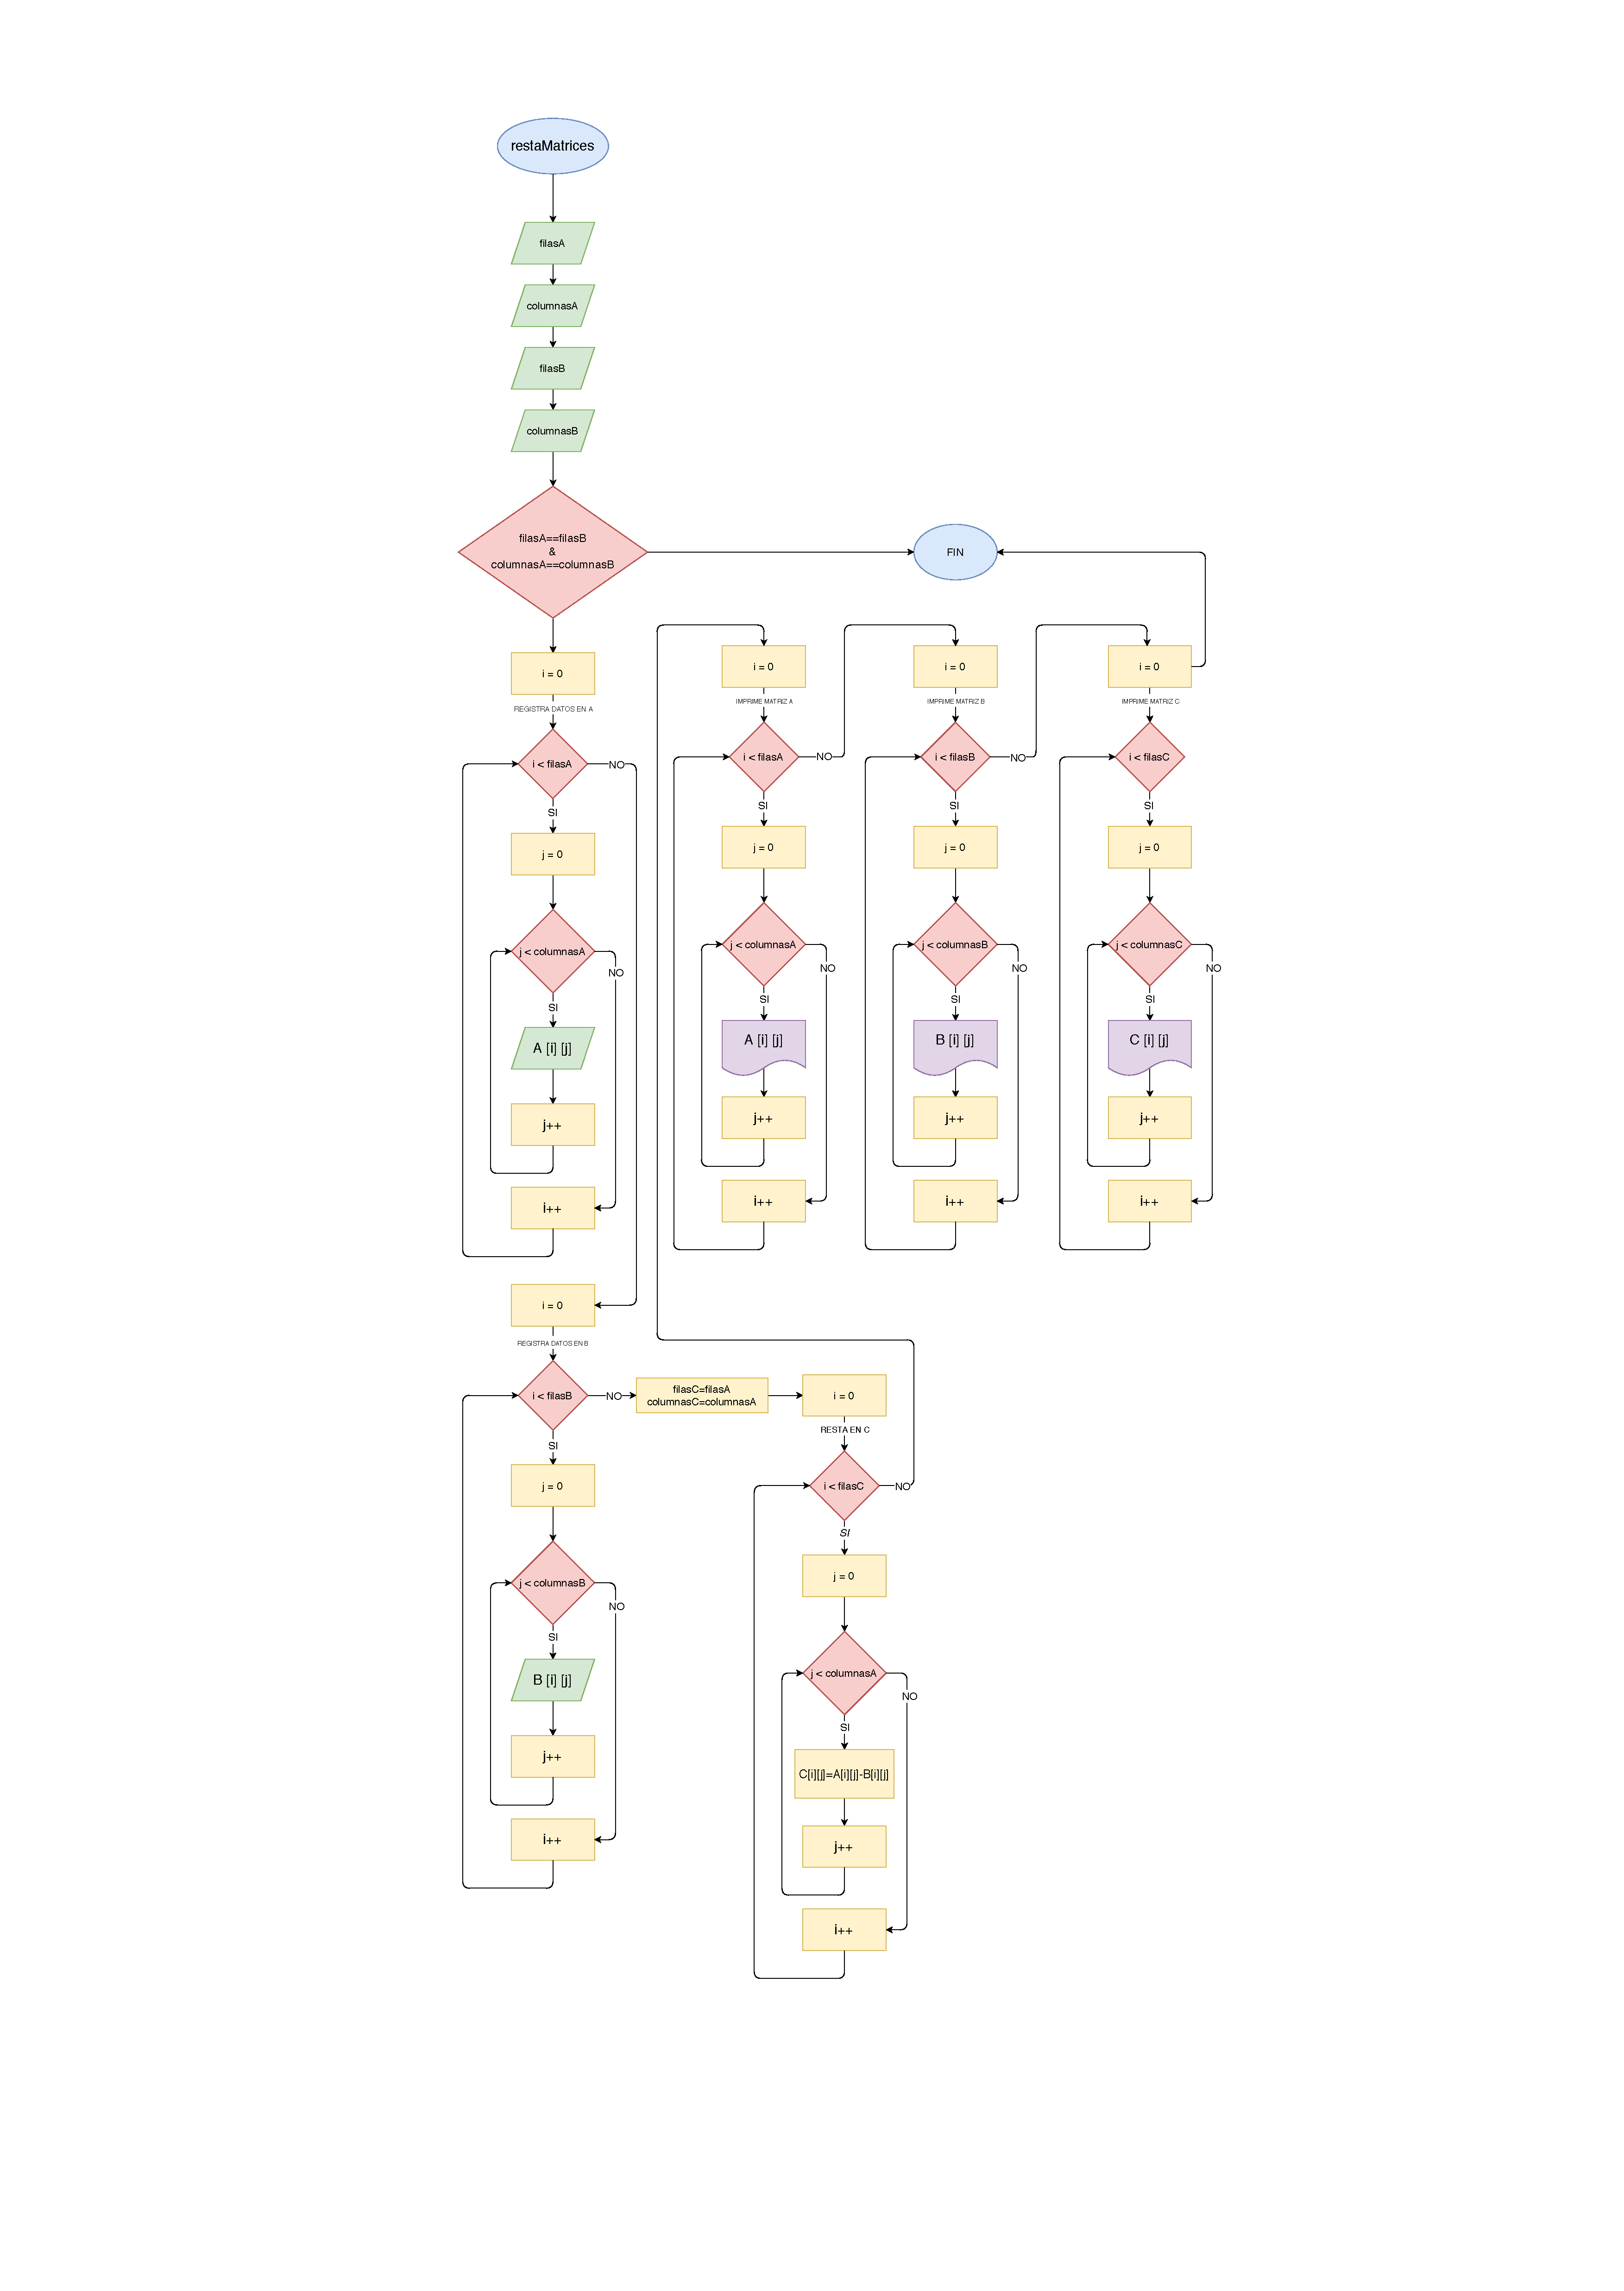
\includegraphics[scale=0.3]{Images/Resta.pdf}
 	\captionof{Diagrama 3: }{Función restaMatrices()}
 	\label{figura4}
 \end{center}
 
\clearpage
\subsection{Diagrama función multiplicacionMatrices ()}
\begin{center}
 	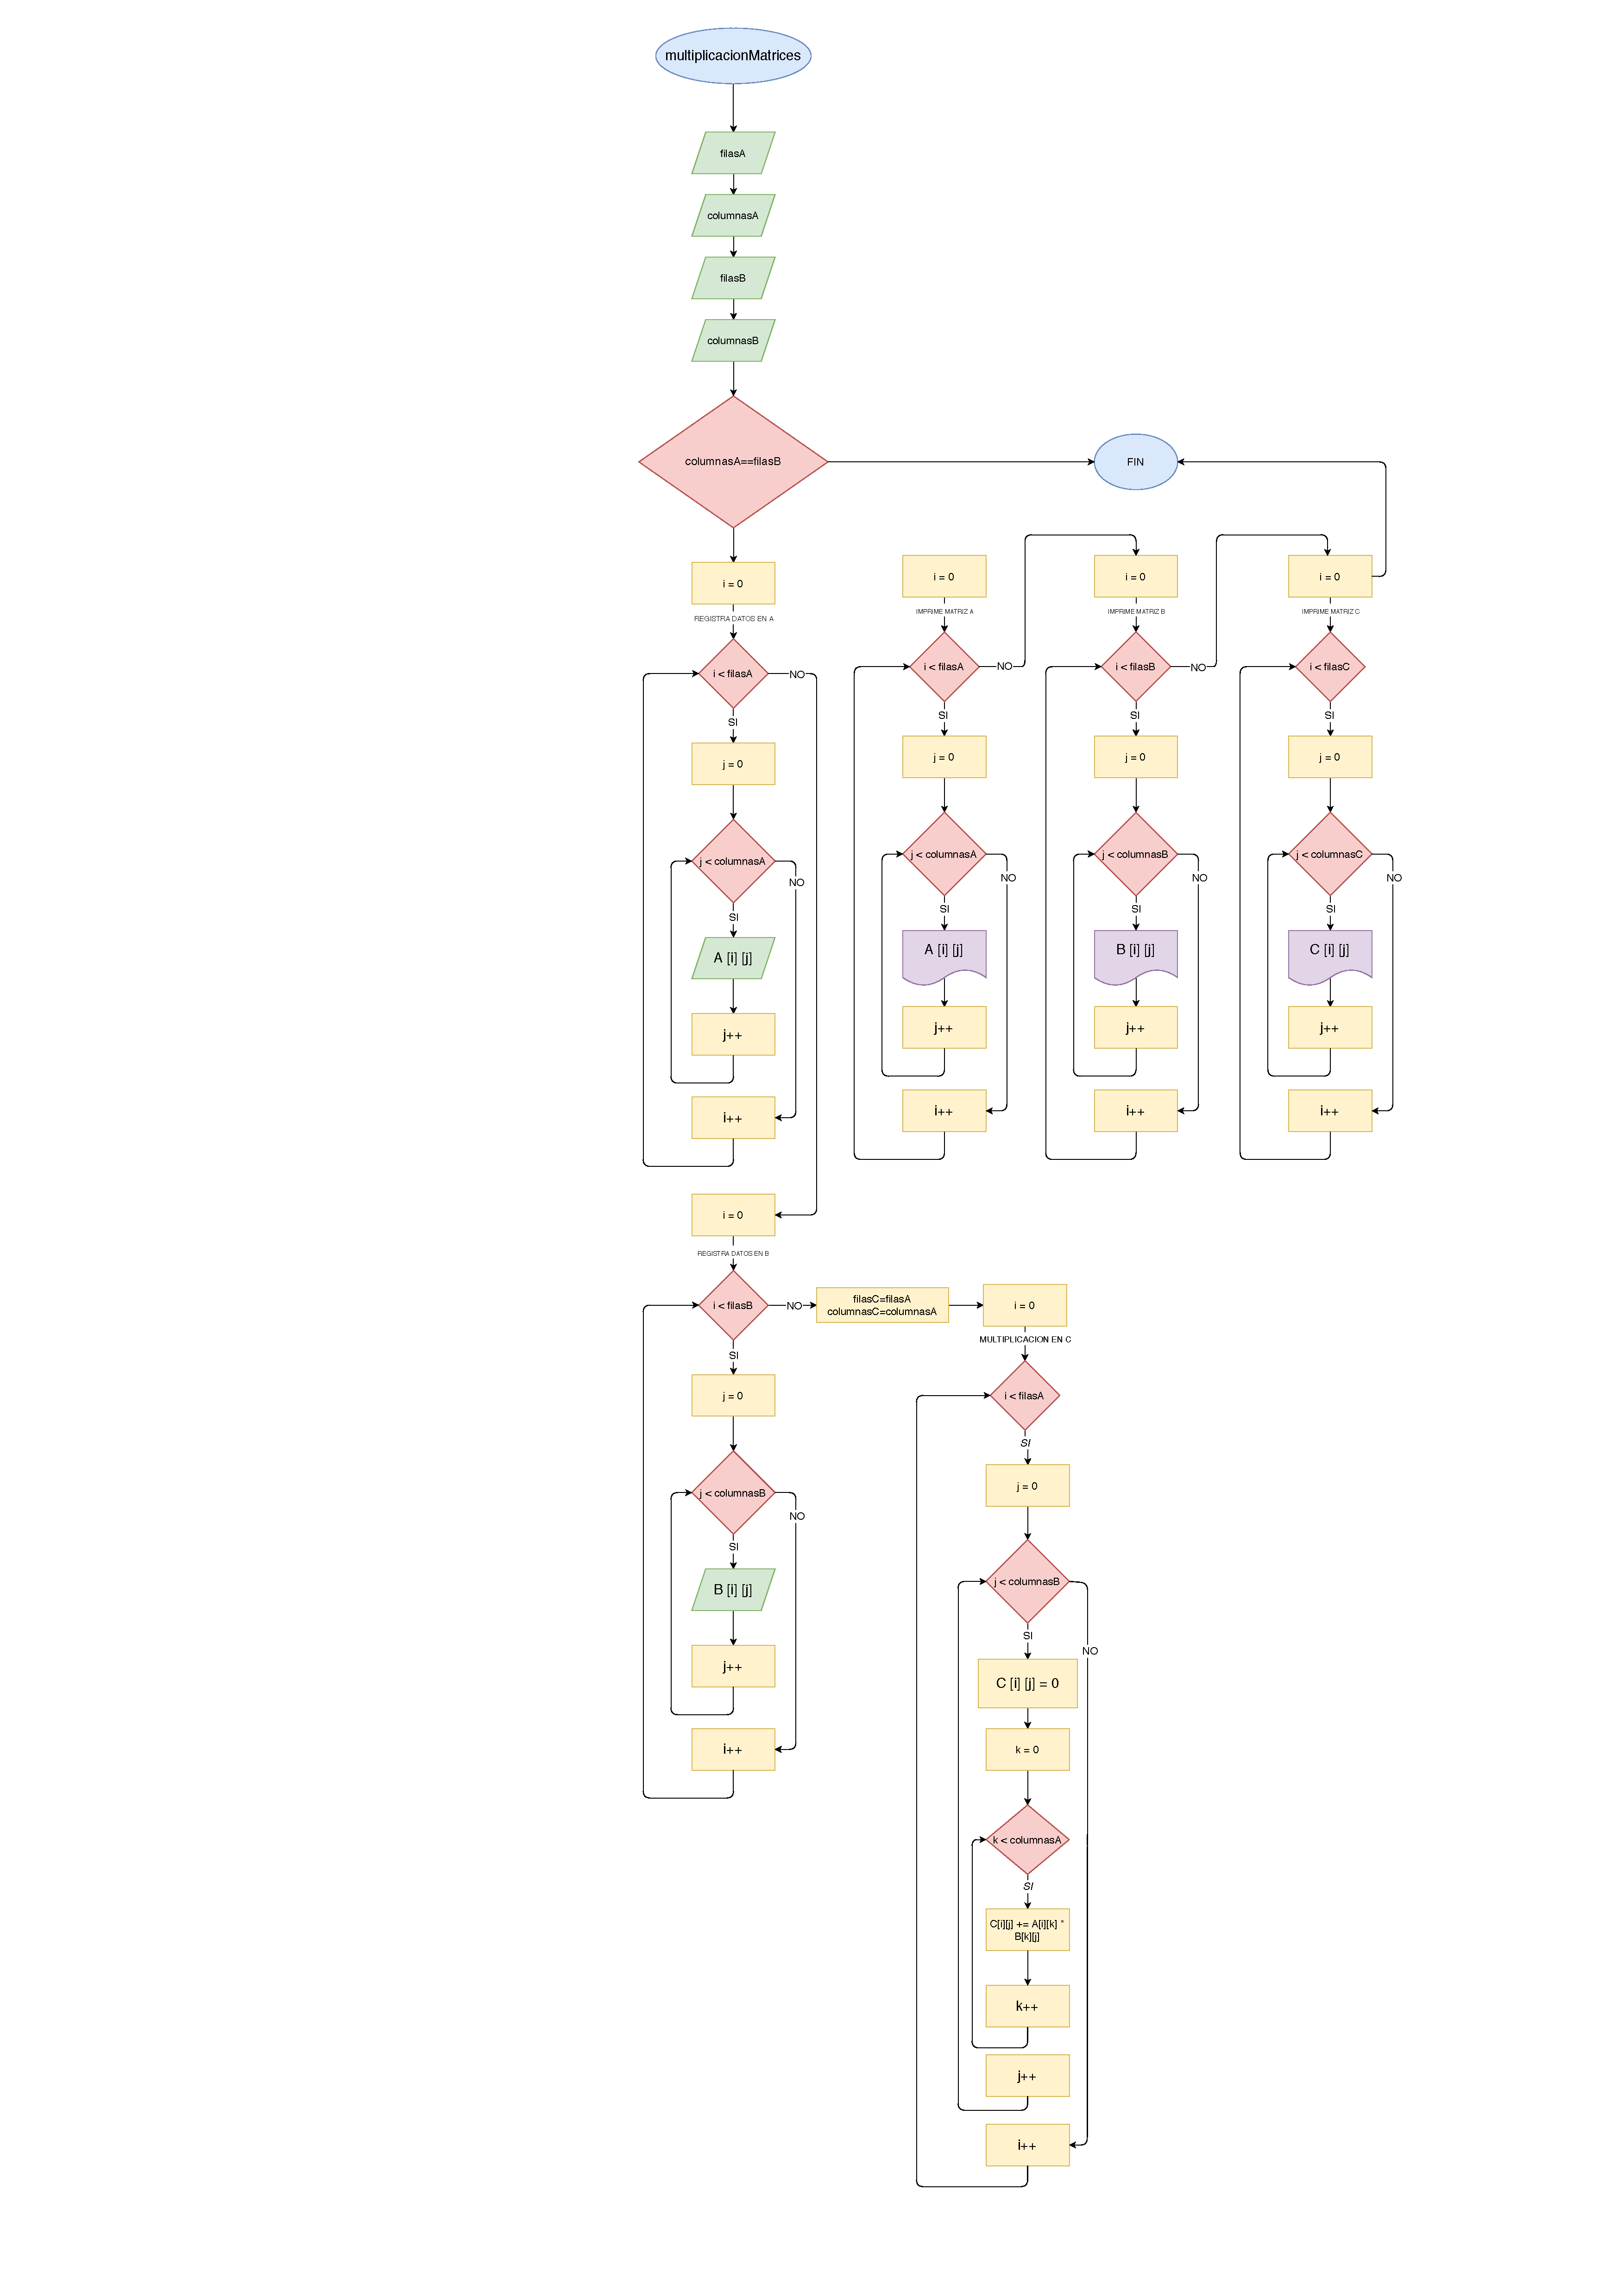
\includegraphics[scale=0.3]{Images/Multiplicacion.pdf}
 	\captionof{Diagrama 4: }{Función multiplicacionMatrices()}
 	\label{figura4}
 \end{center}
\clearpage


\subsection{Diagrama función transpuesta ()}

\begin{center}
 	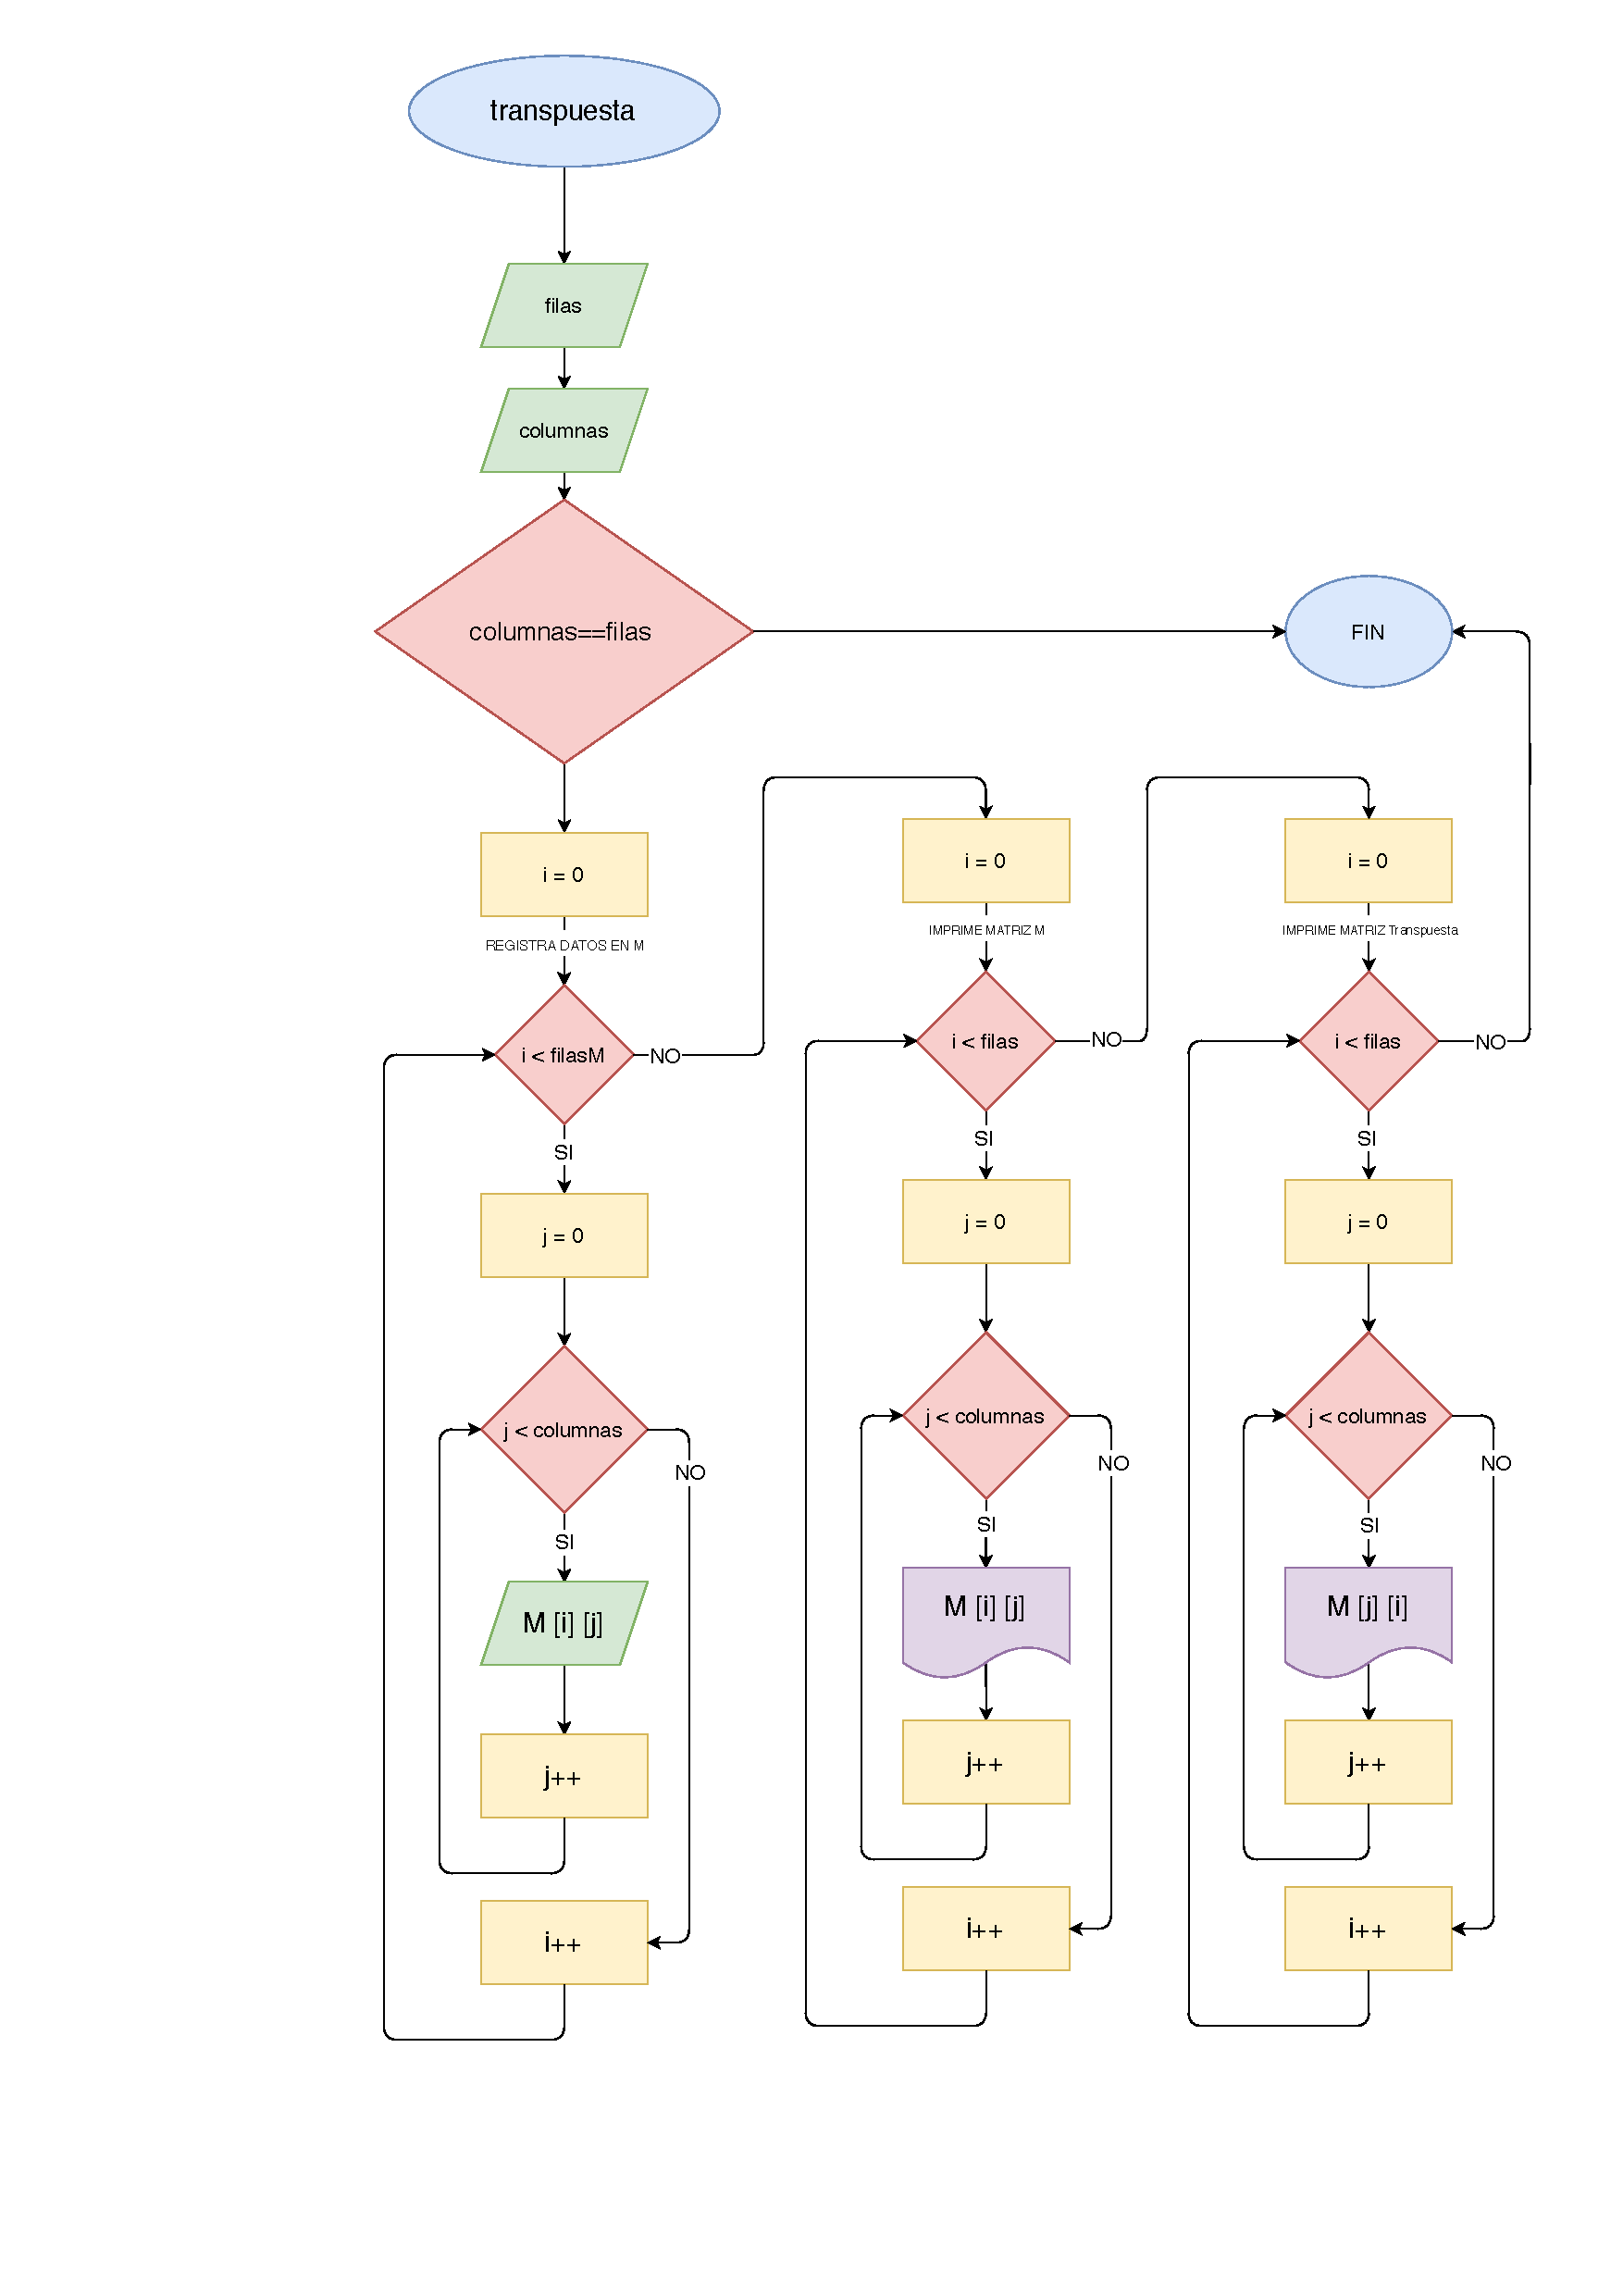
\includegraphics[scale=0.6]{Images/Transpuesta.pdf}
 	\captionof{Diagrama 5: }{Función transpuesta()}
 	\label{figura4}
 \end{center}
\clearpage

\section{Implementación y pruebas}
 

\section{Código fuente comentado}


\lstinputlisting[language=C++]{main.cpp}


\section{Conclusiones}


\section{Bibliografía}
\begin{itemize}
    \item Grossman, S. I. (2008). Álgebra lineal. McGraw Hill Educación.
\end{itemize}



\end{document}